% Grafo de poses global da fusão (GPO.py).
% Compilar sozinho: pdflatex grafo_poses_global.tex
% Na dissertação: \usepackage{standalone} + \includestandalone[width=\linewidth]{figuras/grafo_poses_global}
\documentclass[tikz,border=4pt]{standalone}
\usepackage[T1]{fontenc}
\usepackage[utf8]{inputenc}
\usepackage{amsmath,amssymb,bm}
\usetikzlibrary{calc}

\definecolor{cPrior}{HTML}{0B0B0B}
\definecolor{cVO}{HTML}{2A78D6}
\definecolor{cRoda}{HTML}{EDA100}
\definecolor{cEscala}{HTML}{8A8984}
\definecolor{cLaco}{HTML}{6250D6}

\begin{document}
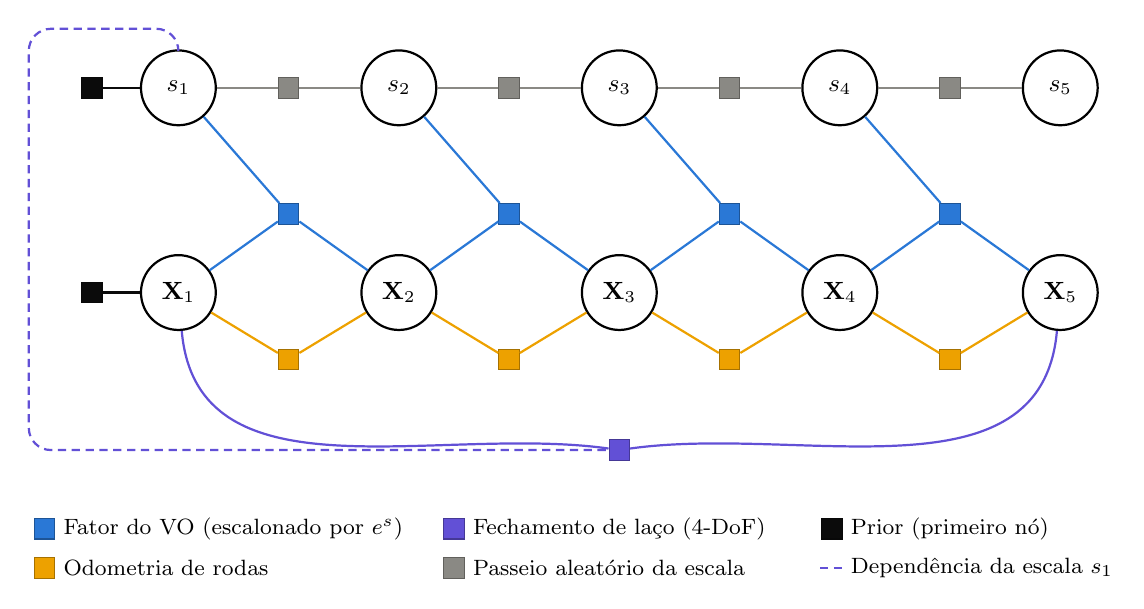
\begin{tikzpicture}[
    font=\small,
    var/.style={circle, draw, thick, minimum size=9.5mm, inner sep=0pt},
    fat/.style={rectangle, fill=#1, draw=#1!70!black, minimum size=2.6mm, inner sep=0pt},
    lig/.style={draw=#1, line width=0.8pt},
    leg/.style={font=\footnotesize, anchor=west, inner sep=1pt},
  ]

  % ---- variáveis: pose do veículo X e log da escala do VO s, um par por nó
  \foreach \n in {1,...,5} {
    \pgfmathsetmacro\x{2.8*(\n-1)}
    \node[var] (X\n) at (\x,0)   {$\mathbf{X}_{\n}$};
    \node[var] (S\n) at (\x,2.6) {$s_{\n}$};
  }

  % ---- priors no primeiro nó (unários)
  \foreach \v in {X1, S1} {
    \node[fat=cPrior] (p\v) at ($(\v)+(-1.1,0)$) {};
    \draw[lig=cPrior] (\v) -- (p\v);
  }

  % ---- passeio aleatório da escala
  \foreach \a/\b in {1/2, 2/3, 3/4, 4/5} {
    \path (S\a) -- (S\b) node[midway, fat=cEscala] (e\a\b) {};
    \draw[lig=cEscala] (S\a) -- (e\a\b) -- (S\b);
  }

  % ---- fator do VO (X_a, X_b, s_a): translação do VO multiplicada por exp(s_a)
  \foreach \a/\b in {1/2, 2/3, 3/4, 4/5} {
    \node[fat=cVO] (v\a\b) at ($(X\a)!0.5!(X\b)+(0,1.0)$) {};
    \draw[lig=cVO] (X\a) -- (v\a\b) -- (X\b);
    \draw[lig=cVO] (v\a\b) -- (S\a);
  }

  % ---- odometria de rodas (métrica)
  \foreach \a/\b in {1/2, 2/3, 3/4, 4/5} {
    \node[fat=cRoda] (w\a\b) at ($(X\a)!0.5!(X\b)+(0,-0.85)$) {};
    \draw[lig=cRoda] (X\a) -- (w\a\b) -- (X\b);
  }

  % ---- fechamento de laço 4-DoF (X_1, X_5, s_1): revisita do lugar do nó 1 no nó 5
  \node[fat=cLaco] (L) at ($(X1)!0.5!(X5)+(0,-2.0)$) {};
  \draw[lig=cLaco] (X1) to[out=-85, in=172] (L);
  \draw[lig=cLaco] (X5) to[out=-95, in=8] (L);
  \draw[lig=cLaco, densely dashed, rounded corners=8pt]
    (S1.north) |- (-1.9,3.35) |- (L.west);

  % ---- legenda (3 colunas)
  \begin{scope}[shift={(-1.7,-3.0)}]
    \node[fat=cVO]     at (0,0)      {}; \node[leg] at (0.2,0)     {Fator do VO (escalonado por $e^{s}$)};
    \node[fat=cRoda]   at (0,-0.5)   {}; \node[leg] at (0.2,-0.5)  {Odometria de rodas};
    \node[fat=cLaco]   at (5.2,0)    {}; \node[leg] at (5.4,0)     {Fechamento de laço (4-DoF)};
    \node[fat=cEscala] at (5.2,-0.5) {}; \node[leg] at (5.4,-0.5)  {Passeio aleatório da escala};
    \node[fat=cPrior]  at (10.0,0)   {}; \node[leg] at (10.2,0)    {Prior (primeiro nó)};
    \draw[lig=cLaco, densely dashed] (9.85,-0.5) -- (10.15,-0.5);
    \node[leg] at (10.2,-0.5) {Dependência da escala $s_1$};
  \end{scope}
\end{tikzpicture}
\end{document}
